\section{Temperature Profiles}
Radial and axial temperature profiles were computed for the cold geometry to verify the profile's shape and to ensure that the calculated values were reasonable.

A temperature map of the fuel rod was created. For each node along the axial direction, the temperature increase in the coolant was first computed based on the heat generated in the fuel. Using this, the temperature at the coolant-cladding interface was determined by applying the heat transfer coefficient, calculated from provided correlations.

For the cladding, a linear temperature profile was assumed to estimate the temperature at the cladding-gas interface. For the gap and the fuel, multiple temperature points were calculated along the radial direction. At each step, the material properties were updated to reflect the temperature of the previous step. The inner void was assumed to be at the same temperature as the inner surface of the fuel.

The results provided an initial validation of the temperature distribution behavior, confirming that the trends were consistent and the values were within expected ranges before proceeding with further analysis.

Figure~\ref{fig:axial_temp_profile} illustrates the axial temperature profile at the interfaces, while Figure~\ref{fig:radial_temp_profile} shows the radial temperature profiles at the bottom, middle, and top of the fuel rod.

\begin{figure}[H]
\centering
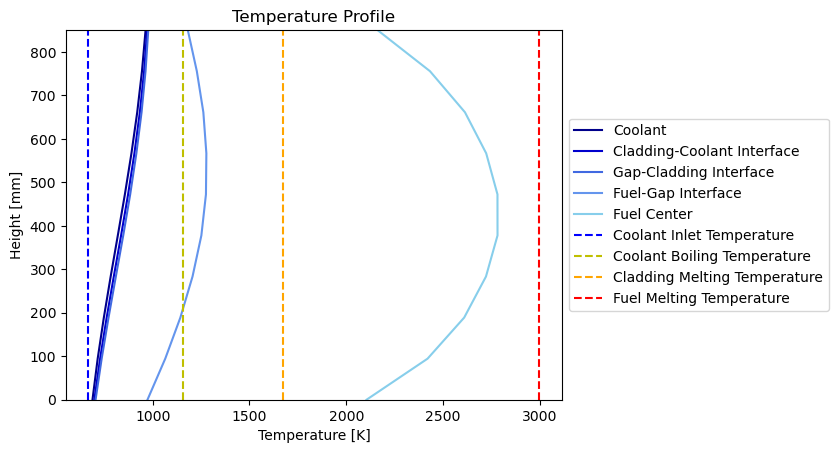
\includegraphics[width=0.7\textwidth]{axial_temp_profile_cold.png}
\caption{Axial temperature profile for cold geometry.}
\label{fig:axial_temp_profile}
\end{figure}

\begin{figure}[H]
\centering
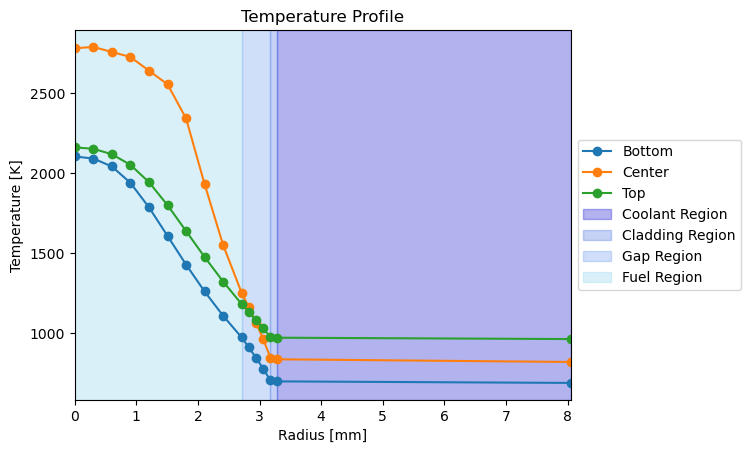
\includegraphics[width=0.7\textwidth]{radial_temp_profile_cold.png}
\caption{Radial temperature profiles for cold geometry at the bottom, middle, and top of the fuel rod.}
\label{fig:radial_temp_profile}
\end{figure}
